%-----------------------------------------------------------------------------
% Template for AIMS- Ghana Structured Masters Research Project
%
% The fonts, linespacing, numbering, page styles, order
% of  Title/Abstract/TOC/Body/{Appendices}/Acknowledgements/References 
% are prescribed as the AIMS house style.
%
% Do not change them or add to it without getting approval first.
% Essays are not accepted if they do not follow house style.
% This is in preparation for your Masters/PhD where the university
% will be much more strict on the house style.
%
\documentclass{aimsessay}
\usepackage[utf8]{inputenc}
\usepackage[round]{natbib}
\setlength{\arrayrulewidth}{1mm}
\setlength{\tabcolsep}{18pt}
\renewcommand{\arraystretch}{1.5}
\usepackage{etoolbox}
%
%-----------------------------------------------------------------------------
% To use external packages for specific needs, 
% get approval before adding them here (they
% should not override general AIMS house style and layout).
%
% Examples:
%
% For Arabic
%\usepackage{arabtex}
\usepackage{arabtex}
{\makeatletter\long\gdef\@gobble#1{}}
\usepackage{utf8}
\setcode{utf8}
% For tables:
\usepackage{booktabs} % \toprule, \midrule, \bottomrule
\usepackage{array}    % \newcolumntype
% 
% For figures:
\usepackage[below]{placeins} % use \FloatBarrier in the body
% \usepackage{float}  %"H" placement spec, for **really here** (i.e. not float)
\usepackage{caption} %many figures in one figure (note subfigure and subfig are deprecated)
\usepackage{subcaption} %many figures in one figure (note subfigure and subfig are deprecated)
%
% For code and algorithms
\usepackage{moreverb}   % \verbatimtabinput
% For links and hyper references
\usepackage{hyperref}
\urlstyle{same}
% \usepackage{listings} % more flexible and complicated 
                        % than moreverb and algorithm

% Others
% \usepackage[all]{xy} 
% \usepackage{sagetex}
% \usepackage{siunitx} % to typeset numbers, units, align decimals in tables.
% \usepackage{dcolumn} % less flexible but maybe faster than siunitx above.
% \usepackage{mathtools} % More maths, e.g. \mathclap.
\usepackage{epstopdf}
\usepackage{psfrag}
\usepackage{graphics}% Others may be landscape, longtable, algorithm, algorithmic, etc.
\usepackage{lineno} % This package together with lineno.sty numbers every line. Makes it easy for edditing.
\usepackage[linesnumbered,ruled]{algorithm2e}
% Numbers lines
%\linenumbers
% 
% ----------------------------------------------------------------------------
% An AIMS Essay can use the sectioning commands "\chapter", "\section",
% "\subsection". No "\subsubsection", "\paragraph", etc. They are disabled.
% 
% For Theorems and such, use the environments defined here:
% \begin{thm}...\end{thm} (or "lem", "defn", etc)
% 
% We put the number to the left of the Theorem heading.
\swapnumbers 
% 
% Theorems are in italics.
\theoremstyle{plain}
\newtheorem{thm}[subsection]{Theorem}
%
% Rest is not in italics.
\theoremstyle{definition} 
\newtheorem{lem}[subsection]{Lemma}
\newtheorem{cor}[subsection]{Corollary}
\newtheorem{conj}[subsection]{Conjecture}
\newtheorem{pro}[subsection]{Proposition}
\newtheorem{exa}[subsection]{Example}
\newtheorem{defn}[subsection]{Definition}
\newtheorem{rem}[subsection]{Remark}
% 
% If you have no theorems, but a lot of equations, maybe the
% following two lines are good. Beware of corresponding Equation
% and Example numbers though! Number equations by sections.
% 
\numberwithin{equation}{section}
%
%-----------------------------------------------------------------------------
% Abstracts are usually written in English, with a version in your
% mother tongue underneath.
%
% French, Twi, Arabic, Malagasy, etc. students use normal LaTeX
% for special characters, for example \'{e}
%
% Amharic students use LibreOffice to write Amharic,
% export and include a figure.
%
%\begin{RLtext}    
%Here is where the arabic text goes.
%You can just type it with an arabic keyboard
%\end{RLtext}\\
%-----------------------------------------------------------------------------
 
% Your own command shortcuts can go here
% keep them clearly separate from other sections of the preamble
% It is good style to have only a few of these so that
% we can read one another's code. If you have to many, 
% then your code does not compile in someone else's template easily,
% and it makes it harder to read. These definitions are only
% meant for very often-used commands to save typing; Examples:
%
%\newcommand {\be}{\begin{equation}}
%\newcommand {\ee}{\end{equation}}
%\newcommand {\C}{\mathbb{C}} % Complex
%\newcommand {\Z}{\mathbb{Z}} % Integers
%\newcommand {\R}{\mathbb{R}} % Real
%\DeclareMathOperator{\sech}{sech} % declaring new math operators like \sin.
%  
%-----------------------------------------------------------------------------
% Title & Author
% On this page you must have NO full-word capitalizations, bold, or colour. 
% All AIMS essays per year have the same title page.
% In English your family name is written last, i.e. Firstname LASTNAME
% English Capitalization, not as in some Francophone countries where
% you write LASTNAME, Firstname.
% Put your AIMS email address only please, for consistency,
% not gmail or some other webmail address.
\title{An Introduction to Evolutionary Dynamic}
% Your name must be in CAPITAL with no comma, 
% and the Family name comes last.
\author{By\\ [1cm]
Dr. Matteo Smelack (matteo@mis.mpg.de)\\
% Igbo, French students, put your special characters above.
% Arabic students can add their name in Arabic letters below, 
% after the english one
% Uncomment the next four lines and edit the name
%%%%%%%%%%%%%%%%%%%%%%%%%%%%%%%%%%%                  
%\begin{RLtext}    
%سشمششة شمثهنعة
%\end{RLtext}\\
%%%%%%%%%%%%%%%%%%%%%%%%%%%%%%%%%%
% Amharic students speak to Jan about how to add your name in your own alphabet.
% Everything here is prescribed; do not enter bold or ALL CAPS here,
% it will not be accepted.
%African Institute for Mathematical Sciences (AIMS) - Ghana\\
% Example1
% Supervised by Professor Barry Green
% University of Stellenbosch, South Africa
% Example2
% Supervised by Doctor Ingrid Rewitzky
% University of Stellenbosch, South Africa
%{\small Supervised by: Title Firstname Lastname}\\
%{\small Institute of Supervisor, Country}%
% Don't put the department, it becomes too long.
}
\date{{\small \today}\\ [0.5cm]
  {\scriptsize\it A short course introducing the theory of Evolutionary dynamic for junior researchers at the Max Planck Institute for Mathematics in the natural Sciences }\\%
  \vspace{3cm}{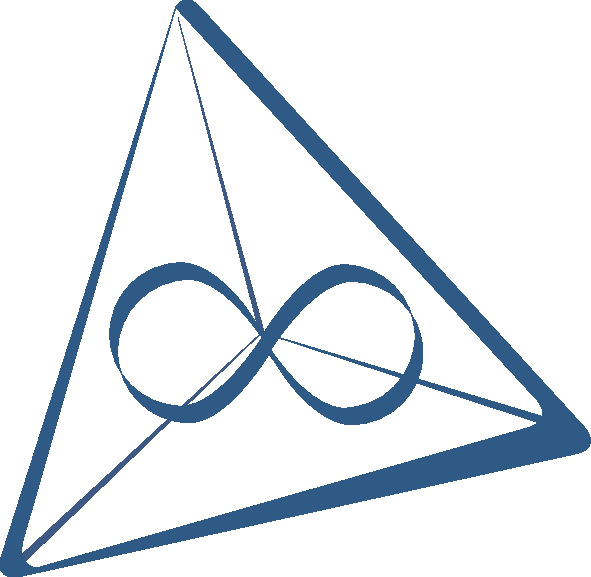
\includegraphics[scale=.3]{images/logo.pdf}}}
%-------------------------------------------------------------------------
\begin{document}
%\selectlanguage{english}
\pagestyle{empty}
\maketitle
% All other files are included via \input. 
% To compile in texmaker while viewing any of those
% without having to switch back, use
%   Options > Define Current Document as 'Master Document'
% To not have to close a PDF, remove viewpdf from quickbuild 
% and open the PDF (once) manually: it will auto-refresh or with control-r
% 
%-------------------------------------------------------------------------
% The abstract is the first thing we want to see. No acknowledgements or 
% dedications here. Fetch the abstract from a separate file.
% Please write it in English and in your mother tongue.
% An abstract should be less than half a page, so that both abstracts 
% (that is both languages) fit onto one page.
% We number roman numerals until the main body
\pagenumbering{roman}
%-----------------------------------------------------------------------------
% See the acknowledgement.tex file and follow the instructions there.
%\chapter*{DECLARATION}
%\addcontentsline{toc}{chapter}{Declaration}
%This work was carried out at AIMS-Ghana in partial fulfilment of the requirements for a Master of Science %Degree.

%I hereby declare that except where due acknowledgement is made, this work has never been presented %wholly or in part for the award of a degree at AIMS-Ghana or any other University.

%\vspace{1.5cm}
%%Please type in your fullname according to the order given and include your electronic signature here%%
%Student: Firstname Middlename Surname 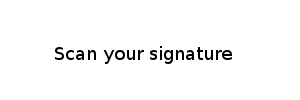
\includegraphics[height=1.5cm]{images/signature.png}

%\vspace{1.5cm}

%%For the supervisor: Please type in your fullname according to the order given and include your electronic signature here%%
%Supervisor: Firstname Middlename Surname 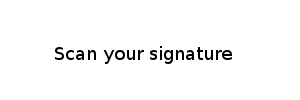
\includegraphics[height=1.5cm]{images/signature1.png}


%\newpage


%\newpage
%\chapter*{DEDICATION} 
%\addcontentsline{toc}{chapter}{Dedication}

%This is optional.

% Abstracts are usually written in English, with a version in your
% mother tongue underneath
\chapter*{Pre-requirements}
\addcontentsline{toc}{chapter}{Pre-requirement}
% Don't change anything above this.
% We do not number this or add it to the contents!
% Overly long acknowledgements are not professional.

\begin{itemize}
	\item Basic statistic and probability 
	\item  Basic Markov process 
	\item Basic differential geometry.
\end{itemize}
{\let\clearpage\relax 

\chapter*{Goals and non-goals} 
\addcontentsline{toc}{chapter}{Goals and non-goals}
% Don't change anything above this.
\hspace*{-1cm}
\large
\begin{tabular}{ |p{8cm}|p{7cm}|  }
	\hline
	\textbf{GOALS}&\textbf{NON-GOALS}\\
	\hline
	Evolution as dynamic&Evolution  as history\\
	Reduction to principle& Explanation of patterns \\
	Intuition & Rigor \\
	Collaboration with some of you& Showing off \\
	\hline
\end{tabular}

}


% At a unviersity like Stellenbosch you *must* produce an abstract in Afrikaans for your masters.
% At AIMS you are encouraged to repeat the abstract in your mother tongue
% French, Igbo, Mlagasy, etc. just write it using LaTeX's special
% characters.
% Arabic students see the arabic.tex file for an example
% Amharic use openoffice and export from there and import a figure here.
% Where the words do not exist put the English work in italics, or use mathematical symbols.





% Don't go typing out the contents.
\tableofcontents
\newpage
% We switch to arabic numerals here where your page count starts
% Essays must be 35 pages long *starting here* and up to and including
% the conclcusion. It does not include the acknowledgements or references.
% 
% Figures may differ between topics, but they are not there
% to fill the pages -- they must add meaning.
% In general most figures should be 0.8 times the width of the page
% (perhaps wider in total when two or three columns of figures)
% See the example in chapter one for defining that. Be *consistent*
% in your presentation of information.
\pagenumbering{arabic}
\pagestyle{myheadings}
%-----------------------------------------------------------------------------
% Each chapter goes in a separate file
% Chapter titles are just examples
% Always have a question
% Note the Case Pattern used at AIMS
\chapter{Selection}
\begin{itemize}
	\item Naive samply vs. evolution 
	\item Notion of fitness 
	\item Dynamics of fitness distributions: 
	\begin{enumerate}
		\item Cumutants and GF 
		\item Asymptotic 
		\item Universality 
		\item Comparison with EVT
	\end{enumerate}
\end{itemize}

\section{Naive sampling}

$n$ components, each with probability $p$,

$$Prob(success)= p^n$$

For $p=\frac{1}{2}$ and $n=100$, $2^{-100}=8\cdot 10^{-31}$ ($1kg/mass$)
\begin{figure}[!h]
% Use "\centering" in floats (figure, table), but if you need to center
% some text (why?) use "\begin{center}...\end{center}".
\centering 
% Figure environments same as 0.8 * \textwidth please
% That does not necessarily mean the actual picture size,
% it is a guideline for the environment which could contain
% 2 or more pictures! Be consistent and follow the guidelines
% provided in your sources.
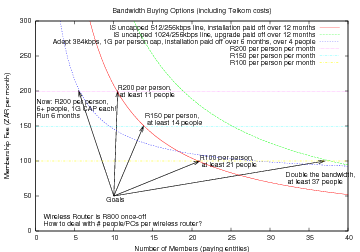
\includegraphics[width=0.8\textwidth]{images/bandwidth-colour.png}
\caption{Planning community bandwidth sharing costs. 
  Note caption capitalization.}
\label{bandwidth} 
% if you move the label it breaks the reference numbering; 
% always have it *after* the caption.
\end{figure}

Remember how to include code with {\tt verbatim} 
and to fix the tabs in {\sf python} in a verbatim environment? 
It may be best to have an `include' command for code, 
not to have to re-edit it all the time.
\verbatimtabinput{code/mycode.py}

\section{Selection: exponential amplification of rare events}

 % Introduction is usually a chapter itself.
\chapter{Mutation}

\section{Global models, Local models }
\begin{algorithm}[H]
 \KwData{this text}
 \KwResult{how to write algorithm with \LaTeX2e }
 initialization\;
 \While{not at end of this document}{
  read current\;
  \eIf{understand}{
   go to next section\;
   current section becomes this one\;
   }{
   go back to the beginning of current section\;
  }
 }
 \caption{How to write algorithms}
\end{algorithm} 
\section{Error thresholds}
\begin{algorithm}
    \SetKwInOut{Input}{Input}
    \SetKwInOut{Output}{Output}
    %\SetKwInOut{Initialisation}{Initialisation}
	
    %\underline{function Euclid} $(a,b)$\;
    \Input{$f_1,f_2,f_3...f_s$ and $<$}
    \Output{$q_1,q_2,q_3...q_s$}
    %\Initialisation{$q_1=q_2=q_3=...=q_s=0$}
    initialization $q_1=q_2=q_3=...=q_s=0$\;
    \While{$v\neq 0$}{
      $i=1$\;
     \While{$i\leq 8$}{
           
    \eIf{$Lt(f_i/Lt(v))$}
      {
        $q_i=q_1 + \frac{Lt(v)}{Lt(f_i)}$\;
         $v=v -\frac{Lt(v)}{Lt(f_i)}f_i$\;
      }
      {
        $i=i+1$\;
      }
      }
      $h = h+Lt(v)$\;
      $v = v-Lt(v)$\;      
      }
    \caption{Division Algorithm}
\end{algorithm}
 % Chapters might go from 2. problem statement, 
                 % through 3. model, to 4. analysis & results
\chapter{Neutrality}

Theorems before the chapter's first section will be dot-zero, 
and their numbering is completely wrong. You can avoid this
by simply always starting a chapter with a section. Ta Da! 
It will probably help you structure your essay anyway. 

\begin{thm}[My Theorem2]
This is my theorem2.
\end{thm}
\begin{proof}
And it has no proof2.
\end{proof}

\section{Neutral evolution as SRW}

Text text text text text text text text text text text text text text
text text text text text text text text text text text text text text
text text text text text text text text text text text text text text
text text text text text text text text text text text text text text
text text text text text.

\begin{thm}[My Theorem2]
This is my theorem2.
\end{thm}
\begin{proof}
And it has no proof2.
\end{proof}

Text text text text text text text text text text text text text text
text text text text text text text text text text text text text text
text text text text text text text text text text text text text text
text text text text text text text text text text text text text text
text text text text text.

\begin{align} % do not use eqnarray. 
\label{2ya}
x & = y + y\\
\label{2yb}
& = 2y
\end{align}
see equations \eqref{2ya} and \ref{2yb}

\section{Neutral evolution as MERW}

Here's a conjecture
\begin{conj}
The washing operation has fixed points.
\end{conj}

and here's an example

\begin{exa}
5 Rand coin.
\end{exa}

 % You do not need to have exactly 4 chapters.
                 % It is probably a good minimum, with 5 chapters 
                 % average, and 7 chapters might be a maximum.
\chapter{Prediction}

An average essay may contain five chapters, but I didn't plan my work properly
and then ran out of time. I spent too much time positioning my figures and worrying
about my preferred typographic style, rather than just using what was provided.
I wasted days bolding section headings and using double slash line endings, and 
had to remove them all again. I spent sleepless nights configuring manually numbered lists
to use the \LaTeX\ environments because I didn't use them from the start or understand
how to search and replace easily with texmaker.

Everyone has to take some shortcuts
at some point to meet deadlines. Time did not allow to test model 
B as well. So I'll skip right ahead and put that under my Future Work section.


\section{Effective potential: dare and dressed suggestions} 
Text text text text text text text text text text text text text text
text text text text text text text text text text text text text text
text text text text text text text text text text text text text text
text text text text text text text text text text text text text text
text text text text text. 

Some essays may have 3, 5 or 6 chapters. This is just an example. 
More importantly, do you have at most 35 pages?  
Luck has nothing to do with it. Use the techniques suggested for
writing your essay.

Now you're demonstrating pure talent and newly acquired skills. 
Perhaps some persistence. Definitely some inspiration. What was that about perspiration? 
Some team work helps, so every now and then why not browse your friends' essays and provide
some constructive feedback?
 % Conclusion is usually a chapter itself. 
%\input{chapter5} % You may have more chapters. (Use e.g. git add FILE)
% This is where we stop counting pages.
% Acknowledgements and References are not counted.
%-----------------------------------------------------------------------------
% Note the errata page is not for now, it is for use during the examination.
% Not that you're going to have any errata.
%-----------------------------------------------------------------------------
% THE BIBLIOGRAPHY 
% Bibliography styles define how the bibliography is 
% listed and formatted. This is part of the AIMS house
% style and is only changed under exceptional circumstances
\renewcommand{\bibname}{References}
\nocite{*}
\bibliographystyle{plainnat}
\bibliography{references}
\addcontentsline{toc}{chapter}{References}
%-----------------------------------------------------------------------------
\end{document}
